% Use xelatex to generate a pdf file of this presentation
%
% OPENING SLIDES ONLY — title + motivation, built with the Funnel Approach:
% wide industry problem -> Postgres-specific mechanism -> one hidden, concrete
% query. The rest of the deck (The Problem / pg_track_optimizer / results)
% continues after the final divider frame below.

\documentclass{beamer}
\usepackage{roboto}
\usepackage[english]{babel}
\usetheme{Copenhagen}

% Aged-paper canvas: the warm off-white of a 1950s typed page.
\definecolor{aged}{HTML}{F6F2E4}
\setbeamercolor{background canvas}{bg=aged}

% Simple way to put a code listing to the slide
\usepackage{listings}

\usepackage{tikz}
\usetikzlibrary{positioning,shapes.geometric,arrows.meta,backgrounds,fadings}
\usepackage{varwidth}  % shrink-to-fit text box for the chapter halo
\usepackage{pgfplots}
\pgfplotsset{compat=1.18}
\usepackage{graphicx}
\usepackage{qrcode}
\usepackage{booktabs}
\usepackage{cancel}

% --- "The Letter" cold-open slide -------------------------------
% Single static page: the wall of text with one line in red.
\usepackage[most]{tcolorbox}
\definecolor{crash}{HTML}{B21F1F}     % swap for pgorange to stay monochrome
\definecolor{paper}{HTML}{FDFAF0}   % sheet on the desk: warmer than the canvas, never pure white
\definecolor{mailrule}{HTML}{D8D6D0}
% one log line: \lgl{ink 0-100}{text}
\newcommand{\lgl}[2]{\textcolor{black!#1}{#2}}
% mail header row
\newcommand{\hdr}[2]{%
  \makebox[1.25cm][l]{\textcolor{black!40}{\tiny\textsf{#1}}}%
  \textcolor{black!75}{\tiny\textsf{#2}}\par}
% ----------------------------------------------------------------

% --- "The Chat" cold-open slide ---------------------------------
% Stylised reproduction of a messenger thread. Light variant so it
% projects well and matches the paper aesthetic of the letter slide.
\definecolor{waoutbg}{HTML}{DCF8C6}   % outgoing (me)
\definecolor{wainbg}{HTML}{FFFFFF}    % incoming (customer)
\definecolor{wabord}{HTML}{E2E2DE}
\definecolor{chatbg}{HTML}{ECE5DD}    % classic chat wallpaper
\definecolor{wablue}{HTML}{34B7F1}    % "read" ticks
% blue double tick
\newcommand{\waticks}{\tikz[x=1pt,y=1pt,baseline=0pt]{%
  \draw[wablue, line width=0.5pt, line cap=round, line join=round]
    (0,2) -- (1.7,0) -- (4.4,3.8);
  \draw[wablue, line width=0.5pt, line cap=round, line join=round]
    (3.0,2) -- (4.7,0) -- (7.4,3.8);}}
% chat header: avatar, redacted contact name, caption
\newcommand{\wahead}[1]{%
  \noindent\raisebox{-1.5pt}{\tikz{\fill[black!22] (0,0) circle (4.5pt);}}%
  \hspace{4pt}%
  \tikz{\fill[black!70, rounded corners=1.5pt] (0,0) rectangle (1.9cm,5.5pt);}%
  \hfill{\tiny\textsf{\textcolor{black!45}{#1}}}\par
  \vspace{2pt}{\color{wabord}\hrule height 0.4pt}\vspace{3pt}}
% centred date pill
\newcommand{\wadate}[1]{%
  \begin{tcolorbox}[enhanced, arc=3pt, colback=wainbg, colframe=wabord,
    boxrule=0.3pt, left=6pt, right=6pt, top=1.5pt, bottom=1pt,
    width=2.7cm, center, before skip=0pt, after skip=3pt]
  \centering\tiny\sffamily\textcolor{black!50}{#1}
  \end{tcolorbox}}
% \wame[width]{time}{text} -- my message, right aligned, with tail + ticks
\newcommand{\wame}[3][0.70]{%
  \begin{tcolorbox}[enhanced, arc=4pt, colback=waoutbg, colframe=wabord,
    boxrule=0.3pt, left=5pt, right=5pt, top=2pt, bottom=1pt,
    width=#1\linewidth, flush right, drop fuzzy shadow=black!10,
    before skip=2pt, after skip=2pt,
    overlay={\fill[waoutbg, draw=wabord, line width=0.3pt]
      ([xshift=-0.6pt]frame.north east) -- ++(5pt,0pt)
        -- ++(-5pt,-6pt) -- cycle;}]
  \footnotesize\sffamily\textcolor{black!85}{#3}%
  \hfill{\tiny\textcolor{black!35}{#2}}\,\waticks
  \end{tcolorbox}}
% \wathem[width]{time}{text} -- customer message, left aligned
\newcommand{\wathem}[3][0.70]{%
  \begin{tcolorbox}[enhanced, arc=4pt, colback=wainbg, colframe=wabord,
    boxrule=0.3pt, left=5pt, right=5pt, top=2pt, bottom=1pt,
    width=#1\linewidth, flush left, drop fuzzy shadow=black!10,
    before skip=2pt, after skip=2pt,
    overlay={\fill[wainbg, draw=wabord, line width=0.3pt]
      ([xshift=0.6pt]frame.north west) -- ++(-5pt,0pt)
        -- ++(5pt,-6pt) -- cycle;}]
  \footnotesize\sffamily\textcolor{black!85}{#3}%
  \hfill{\tiny\textcolor{black!35}{#2}}
  \end{tcolorbox}}
% ----------------------------------------------------------------

% Emblem shown in the corner of every slide, and larger on the title page
% Madrid coat of arms removed for PGDay Israel; restore if needed:
% \logo{\includegraphics[scale=0.08]{pics/madrid_coat_of_arms}}

% Blocks settings
\setbeamerfont{block title}{size=\tiny}
\setbeamertemplate{navigation symbols}{}

%Information to be included in the title page:
% short form for the footer: the full title plus "10 / 10" no longer fits
% Title as published in the PGConf.EU 2026 schedule (session 7926),
% split at the colon into title + subtitle.
% Sentence case, as in the schedule and as the pgEdge Brand Book asks;
% line breaks are placed by hand for the cover (\texorpdfstring keeps
% them out of the PDF metadata).
\title[Finding the invisible]{Finding the\texorpdfstring{\\}{ }invisible}
\subtitle{Spotting query planner issues\texorpdfstring{\\}{ }before they appear}
% eyebrow above the title on the cover
\newcommand{\eventname}{PGConf.EU 2026 \textperiodcentered{} Valencia}
% Easter egg: a tiny flag of the Community of Madrid (crimson, seven white
% stars 4 + 3, 2:3) left of the name in the footline only. Muted crimson so
% it sits quietly in the dark author box; \texorpdfstring keeps it out of
% the PDF metadata.
\definecolor{madridcrimson}{HTML}{B5122B}
\newcommand{\madridflag}{\tikz[x=1pt,y=1pt,baseline=0pt]{%
  \fill[madridcrimson] (0,0) rectangle (6.9,4.6);
  \foreach \x in {1.2,2.7,4.2,5.7} \node[star,star points=5,star point ratio=2.4,
    minimum size=1.15pt,inner sep=0pt,fill=white] at (\x,3.25) {};
  \foreach \x in {1.95,3.45,4.95} \node[star,star points=5,star point ratio=2.4,
    minimum size=1.15pt,inner sep=0pt,fill=white] at (\x,1.35) {};}}
\author[\texorpdfstring{\madridflag\hspace{3pt}}{}Andrei Lepikhov]{Andrei Lepikhov}
\institute{pgEdge}
\date{22 October 2026}

% Add page numbers in the footnote
\expandafter\def\expandafter\insertshorttitle\expandafter{%
  \insertshorttitle\hfill%
  \insertframenumber\,/\,\inserttotalframenumber}

\definecolor{lightlightgray}{gray}{0.9}
\definecolor{pgblue}{HTML}{336791}
\definecolor{pgorange}{HTML}{E8781A}

% --- "One query, two views" slide -------------------------------
\definecolor{ptoink}{HTML}{14213D}      % headings / figures
\definecolor{ptoteal}{HTML}{2B6A6C}     % pg_stat_statements label
\definecolor{ptoaccent}{HTML}{C2410C}   % pg_track_optimizer label, statement bar
\definecolor{ptotint}{HTML}{FDF1EA}     % callout background
\definecolor{ptopaper}{HTML}{FFF8F3}    % text on the statement bar
% ----------------------------------------------------------------

% --- pgEdge-style section divider (pgEdge Brand Book) -------------
% Brand book, section 4: dividers are a light tint (Sky / Mist / Teal 1)
% with ASCII clouds as a full-bleed backdrop and one title at left-middle
% in Night. Navy is kept for the cover and the closing page only, so the
% deck opens and ends dark and every chapter break reads as a pause.
% Tints cycle sky -> mist -> teal, as in the pgedge Beamer theme.
% No negative tracking: brand values are tuned for Metro Sans, not Roboto.
\definecolor{pgeNavy}{HTML}{003E63}
\definecolor{pgeNight}{HTML}{002B44}
\definecolor{pgeSkyMid}{HTML}{A4D7FF}
\definecolor{pgeBlue}{HTML}{1385C7}
\definecolor{pgePath}{HTML}{56716E}  % secondary text on tints
\definecolor{pgeSky}{HTML}{ECF7FF}
\definecolor{pgeMist}{HTML}{F1F4F4}
\definecolor{pgeTeal}{HTML}{CEE9E8}
\newcounter{pgechap}
% \pgechapter{eyebrow}{title, break lines with \\}
\newcommand{\pgechapter}[2]{{%
  \stepcounter{pgechap}%
  \pgfmathtruncatemacro\pgek{mod(\value{pgechap}-1,3)}%
  % One canvas for every chapter: the deck's aged-paper yellow instead of
  % the brand's Sky / Mist / Teal cycle (author's choice, keeps the
  % dividers in the same paper world as the content slides). Only the
  % cloud pattern still varies from chapter to chapter.
  \def\pgebg{aged}%
  \ifcase\pgek\relax
    \def\pgeart{ascii-clouds-a-dark}\def\pgeop{0.35}%
  \or\def\pgeart{ascii-clouds-c-dark}\def\pgeop{0.35}%
  \or\def\pgeart{ascii-clouds-b-dark}\def\pgeop{0.35}%
  \fi
  \setbeamertemplate{background}{%
    \begin{tikzpicture}[x=1pt,y=1pt]
      \useasboundingbox (0,0) rectangle (\paperwidth,\paperheight);
      \clip (0,0) rectangle (\paperwidth,\paperheight);
      \begin{scope}[on background layer]
        \fill[\pgebg] (0,0) rectangle (\paperwidth,\paperheight);
        % 16:9 clouds on a 4:3 page: full height, centred, sides trimmed by the page
        \node[inner sep=0,opacity=\pgeop] at (0.5\paperwidth,0.5\paperheight)
          {\includegraphics[height=\paperheight]{pgedge-assets/\pgeart}};
      \end{scope}
      \node[anchor=west,inner sep=0] (pgetxt) at (8mm,0.5\paperheight) {%
        \begin{varwidth}{0.66\paperwidth}\raggedright
        {\sffamily\bfseries\fontsize{8}{10}\selectfont\color{pgeBlue}%
         \addfontfeatures{LetterSpace=8}\MakeUppercase{#1}\par}%
        \vskip3.5mm
        {\sffamily\bfseries\fontsize{32}{32}\selectfont\color{pgeNight}%
         \spaceskip=0.32em\relax\hyphenpenalty=10000 #2\par}%
        \end{varwidth}};
      % Calm zone: a halo in the page's own tint, drawn above the clouds and
      % below the text. Solid over the text, fading out at the edges, so it
      % reads as "the clouds part here", not as a box.
      \begin{scope}[on background layer]
        \path let \p1 = ($(pgetxt.north east)-(pgetxt.center)$),
                  \n1 = {1.55*\x1+14mm}, \n2 = {1.55*\y1+12mm} in
          [fill=\pgebg, path fading=circle with fuzzy edge 20 percent]
          ($(pgetxt.center)-(\n1,\n2)$) rectangle ($(pgetxt.center)+(\n1,\n2)$);
      \end{scope}
    \end{tikzpicture}}%
  \begin{frame}[plain]\end{frame}}}
% ----------------------------------------------------------------

% --- Query plans as graphs (planslides.sty, from the plan-template session)
% Keep the deck's own fonts; re-tint the plan boxes to the paper palette.
\usepackage[nomonofont]{planslides}
\colorlet{planbg}{paper}
\colorlet{planrule}{mailrule}
\colorlet{planbad}{crash}
\colorlet{plantext}{ptoink}
\renewcommand\planedgewidth{0.7pt}   % plan-graph edges
% plan box that stands out from its neighbours: red frame, warm tint inside
\makeatletter
\newenvironment{planhot}
  {\VerbatimEnvironment
   \begin{plan@frame}[colframe=crash, boxrule=0.8pt, colback=ptotint]%
   \plan@fv\begin{Verbatim}}
  {\end{Verbatim}\end{plan@frame}}
\makeatother
% SQL highlighting inside sql/psql boxes (commandchars are on there)
\newcommand\kw[1]{\textcolor{pgblue}{#1}}       % keyword
\newcommand\sqlnum[1]{\textcolor{ptoaccent}{#1}} % numeric literal
\newcommand\sqlcmt[1]{\textcolor{planfade}{#1}}  % -- comment

% fact cards for a tcbraster: big headline + one line of explanation
\newcommand{\factcard}[3][ptoink]{%
  \begin{tcolorbox}[colframe=#1]
  {\sffamily\huge\bfseries\color{#1}#2}\par\smallskip
  {\sffamily\small\color{ptoink}\raggedright\hyphenpenalty=10000 #3\par}
  \end{tcolorbox}}
% ----------------------------------------------------------------

% Default listing format
\lstset{language=sql, frame=none, tabsize=2, identifierstyle=\color{black},
  showspaces=false, showtabs=false, showstringspaces=false,
  columns=fullflexible, % Restore default spaces between letters
  basicstyle=\rmfamily\scriptsize,
  stringstyle=\color{purple},
  keywordstyle=\bfseries\color{green!40!black},
  numberstyle=\tiny\color{gray},
  morekeywords={PUBLICATION,SUBSCRIPTION,CONNECTION,WITH,COPY,FORMAT}}

% -----------------------------

\begin{document}

% %%%%%%%%%%%%%%%%%%%%%%%%%%%%%%%%%%%%%%%%%%%%%%%%%%%%%%%%%%%%%%%%%%%%%%%%
% Title
% %%%%%%%%%%%%%%%%%%%%%%%%%%%%%%%%%%%%%%%%%%%%%%%%%%%%%%%%%%%%%%%%%%%%%%%%

% pgEdge Brand Book "Cover" archetype (cf. \pgtitleframe in the pgedge
% theme), redrawn for this 4:3 Copenhagen deck: full-bleed navy, ASCII
% swirl at 35% cropped by the right edge, logo top-left, SkyMid eyebrow,
% white SemiBold title, SkyMid subtitle, speaker block bottom-left.
% Roboto stays: Metro Sans is not installed, and the brand's negative
% tracking is tuned for Metro Sans only.
{\setbeamertemplate{background}{%
  \begin{tikzpicture}[x=1pt,y=1pt]
    \useasboundingbox (0,0) rectangle (\paperwidth,\paperheight);
    \fill[pgeNavy] (0,0) rectangle (\paperwidth,\paperheight);
    \node[anchor=east,inner sep=0,opacity=0.35]
      at ([xshift=34mm]\paperwidth,0.5\paperheight)
      {
\includegraphics[height=0.92\paperheight]{pgedge-assets/ascii-swirl-light}};
    \node[anchor=north west,inner sep=0] at (8mm,\paperheight-8mm)
      {
\includegraphics[height=4.5mm]{pgedge-assets/logo-on-dark}};
    \node[anchor=west,inner sep=0,text width=0.72\paperwidth,align=left]
      at (8mm,0.53\paperheight) {\hyphenpenalty=10000\exhyphenpenalty=10000
      {\sffamily\bfseries\fontsize{7}{9}\selectfont\color{pgeSkyMid}%
       \addfontfeatures{LetterSpace=8}\MakeUppercase{\eventname}\par}%
      \vskip3.5mm
      {\sffamily\bfseries\fontsize{28}{30}\selectfont\color{white}%
       \spaceskip=0.32em\relax\inserttitle\par}%
      \vskip4mm
      {\sffamily\fontsize{13}{15.5}\selectfont\color{pgeSkyMid}%
       \insertsubtitle\par}};
    \node[anchor=south west,inner sep=0,text width=0.6\paperwidth,align=left]
      at (8mm,8mm) {\spaceskip=0.25em\relax
      {\sffamily\bfseries\fontsize{9}{11.5}\selectfont\color{white}%
       \insertauthor\par}%
      {\sffamily\fontsize{9}{11.5}\selectfont\color{pgeSkyMid}%
       \insertdate\par}};% institute omitted: the logo already says pgEdge
  \end{tikzpicture}}
\begin{frame}[plain,noframenumbering]\end{frame}}

% %%%%%%%%%%%%%%%%%%%%%%%%%%%%%%%%%%%%%%%%%%%%%%%%%%%%%%%%%%%%%%%%%%%%%%%%
% Section divider: "Origins of the idea", pgEdge brand style (see
% \pgechapter in the preamble): light tint, ASCII clouds at 35-40%
% opacity, "Chapter 1" eyebrow over a two-line title. Opens the
% cold-open pair below (the letter + the chat).
% %%%%%%%%%%%%%%%%%%%%%%%%%%%%%%%%%%%%%%%%%%%%%%%%%%%%%%%%%%%%%%%%%%%%%%%%

\pgechapter{Chapter 1}{Origins\\of the idea}

% %%%%%%%%%%%%%%%%%%%%%%%%%%%%%%%%%%%%%%%%%%%%%%%%%%%%%%%%%%%%%%%%%%%%%%%%
% Cold open: the letter that started the investigation
% %%%%%%%%%%%%%%%%%%%%%%%%%%%%%%%%%%%%%%%%%%%%%%%%%%%%%%%%%%%%%%%%%%%%%%%%

\begin{frame}[fragile]\frametitle{31 December 2023}

\vspace{-0.9em}

\begin{tcolorbox}[
  enhanced, sharp corners=downhill, arc=1pt,
  colback=paper, colframe=mailrule, boxrule=0.4pt,
  left=6pt, right=6pt, top=5pt, bottom=2pt,
  drop shadow={black!12}]

\hdr{From}{Xxxxxxxx X. Xxxxxxx
           \textcolor{black!35}{$\langle$xxxxxxxxxxxxxx@xxxxxx.com$\rangle$}}
\hdr{Subject}{\textbf{Segmentation fault caused by Postgrest -
              reateplan.c:6178 - prepare\_sort\_from\_pathkeys}}

\vspace{-1pt}\textcolor{mailrule}{\hrule height 0.4pt}\vspace{6pt}

{\ttfamily\fontsize{6.8}{9.0}\selectfont
 \setlength{\parskip}{0pt}\setlength{\topsep}{0pt}\setlength{\partopsep}{0pt}
\begin{semiverbatim}
\lgl{62}{2023-12-31 03:23:12.048 PST [17763] LOG: server process (PID 19014) was}
\lgl{62}{terminated by \textcolor{crash}{signal 11: Segmentation fault}}
\lgl{62}{2023-12-31 03:23:12.048 PST [17763] DETAIL: Failed process was running:}
\lgl{50}{      with recursive}
\lgl{48}{      pks_fks as (}
\lgl{34}{        -- pk + fk referencing col}
\lgl{44}{        select}
\lgl{40}{          contype::text as contype,}
\lgl{36}{          conname,}
\lgl{31}{          array_length(conkey, 1) as ncol,}
\lgl{26}{          conrelid as resorigtbl,}
\lgl{21}{          col as resorigcol,}
\lgl{16}{          ord}
\lgl{12}{        from pg_constraint}
\lgl{8}{        left join lateral unnest(conkey) with ordinality as _(col, ord)}
\lgl{4}{        where contype IN ('p', 'f')}
\end{semiverbatim}
}
\end{tcolorbox}

\end{frame}

% %%%%%%%%%%%%%%%%%%%%%%%%%%%%%%%%%%%%%%%%%%%%%%%%%%%%%%%%%%%%%%%%%%%%%%%%
% Cold open, part two: the chat with the user who rolled it out anyway
% %%%%%%%%%%%%%%%%%%%%%%%%%%%%%%%%%%%%%%%%%%%%%%%%%%%%%%%%%%%%%%%%%%%%%%%%

\begin{frame}\frametitle{12 January 2024}

\vspace{-0.7em}

\begin{tcolorbox}[enhanced, sharp corners, colback=chatbg, colframe=chatbg,
  boxrule=0pt, left=5pt, right=5pt, top=3pt, bottom=3pt,
  before skip=0pt, after skip=0pt]

\wahead{private chat with an AQO user (sensitive information hidden)}

\wadate{12 Jan 2024}

\wame[0.86]{1:41}{Be careful using AQO -- just remember, AI guesses, and
  these predictions can sometimes be totally wrong. The best results I
  achieved were when I used it manually, correcting only specific
  problematic queries.}

\wathem[0.68]{3:06}{We have turned on AQO across
  \textcolor{crash}{\textbf{5\,000 servers}} for all queries now}

\wathem[0.26]{3:06}{We love it.}

\wame[0.62]{3:07}{Do you have some positive effect?}

\wathem[0.19]{3:15}{Yes.}

\wathem[0.52]{3:15}{Much faster across the board.}

\wathem[0.72]{3:18}{I.e.\ run the query 50\% time without AQO then
  50\% w/ AQO then compare}

\end{tcolorbox}

\end{frame}

% %%%%%%%%%%%%%%%%%%%%%%%%%%%%%%%%%%%%%%%%%%%%%%%%%%%%%%%%%%%%%%%%%%%%%%%%
% The takeaway of the cold open
% %%%%%%%%%%%%%%%%%%%%%%%%%%%%%%%%%%%%%%%%%%%%%%%%%%%%%%%%%%%%%%%%%%%%%%%%

\begin{frame}
\vspace*{\fill}
\begin{center}
{\LARGE The query plan is a great source
 of savings on your cloud bill.}

\bigskip
\begin{minipage}{0.86\textwidth}\centering
{\large\textcolor{black!55}{It requires no extra hardware or watts ---
 just a little thought and careful tuning.}}
\end{minipage}
\end{center}
\vspace*{\fill}
\end{frame}

% %%%%%%%%%%%%%%%%%%%%%%%%%%%%%%%%%%%%%%%%%%%%%%%%%%%%%%%%%%%%%%%%%%%%%%%%
% Section divider: "Blind spot" -- same pgEdge style as Chapter 1.
% Opens the part on why misestimation is hard to see in the statistics.
% %%%%%%%%%%%%%%%%%%%%%%%%%%%%%%%%%%%%%%%%%%%%%%%%%%%%%%%%%%%%%%%%%%%%%%%%

\pgechapter{Chapter 2}{Blind spot}

% %%%%%%%%%%%%%%%%%%%%%%%%%%%%%%%%%%%%%%%%%%%%%%%%%%%%%%%%%%%%%%%%%%%%%%%%
% What a real workload looks like (adapted from the PG Bootcamp deck,
% slide "Типичная БД и запросы")
% %%%%%%%%%%%%%%%%%%%%%%%%%%%%%%%%%%%%%%%%%%%%%%%%%%%%%%%%%%%%%%%%%%%%%%%%

\begin{frame}[fragile]\frametitle{Is it easy to spot an optimisation problem?}
\setbeamerfont{itemize/enumerate body}{size=\scriptsize}
\setbeamerfont{itemize item}{size=\scriptsize}

\vspace{-0.4em}
	{\footnotesize\textit{One production ERP database ...}}

\begin{columns}[T]
\begin{column}{0.55\textwidth}
\begin{center}
	{\scriptsize\textbf{Example query}}\par\vspace{2pt}
\end{center}
\begin{tcolorbox}[enhanced, sharp corners=downhill, arc=1pt,
  colback=paper, colframe=mailrule, boxrule=0.4pt,
  left=3pt, right=3pt, top=3pt, bottom=2pt,
  before skip=0pt, after skip=2pt]
\begin{lstlisting}[language=SQL, breaklines=true, columns=fixed,
  basicstyle=\ttfamily\fontsize{3.1}{3.5}\selectfont,
  keywordstyle=\ttfamily]
SELECT T1.Fld100343RRef,
 (CAST(CAST((T16.Fld100345_ * T1.Fld100346_) AS NUMERIC(28,8)) /
 (T16.Fld100346_ * T1.Fld100345_) AS NUMERIC(28,8)))
FROM (SELECT T15._Fld100344RRef AS Fld100344RRef,
 T15._Fld100343RRef AS Fld100343RRef, T15._Fld100346 AS Fld100346_,
 T15._Fld100345 AS Fld100345_
FROM (SELECT T3._Fld100343RRef AS Fld100343RRef,
 T3._Fld100344RRef AS Fld100344RRef, MAX(T3._Period) AS MAXPERIOD_
FROM _InfoRg100342 T3
WHERE ((T3._Fld2488 = CAST(0 AS NUMERIC))) AND (T3._Period <=
 '2023-12-04 12:49:02'::timestamp AND (EXISTS(SELECT 1
FROM pg_temp.tt3319 T4
LEFT OUTER JOIN _Reference101 T5
 ON (T4._Q_001_F_007RRef = T5._IDRRef) AND (T5._Fld2488 = CAST(0 AS NUMERIC))
LEFT OUTER JOIN _Reference395 T6
 ON (T4._Q_001_F_005RRef = T6._IDRRef) AND (T6._Fld2488 = CAST(0 AS NUMERIC))
LEFT OUTER JOIN _Reference366X1 T7
 ON (T4._Q_001_F_006RRef = T7._IDRRef) AND (T7._Fld2488 = CAST(0 AS NUMERIC))
WHERE ((1=1 OR 1=0) AND (T4._Q_001_F_001RRef =
 '\216@\030f\332\261R\333\021\356\222\212\342\004z\226'::bytea) AND
 (T5._Fld53293RRef = '\214\215O\271\351\244\310\000B<\227\003{~\356e'::bytea)
 AND ((T7._Fld59861RRef <> '\201F\nu\257Q\301Fp\027O\211\214\001{'::bytea)
 OR (T7._Fld59861RRef = '\201F\nu\257Q\301Fp\027O\211\214\001{'::bytea)))
 AND ((T3._Fld100343RRef = T5._Fld53297RRef) AND
 (T3._Fld100344RRef = T6._Fld101340RRef))
UNION ALL SELECT 1
FROM pg_temp.tt3319 T8
LEFT OUTER JOIN _Reference101 T9
 ON (T8._Q_001_F_007RRef = T9._IDRRef) AND (T9._Fld2488 = CAST(0 AS NUMERIC))
LEFT OUTER JOIN _Reference101 T10
 ON (T9._Fld53299RRef = T10._IDRRef) AND (T10._Fld2488 = CAST(0 AS NUMERIC))
LEFT OUTER JOIN _Reference395 T11
 ON (T8._Q_001_F_005RRef = T11._IDRRef) AND (T11._Fld2488 = CAST(0 AS NUMERIC))
LEFT OUTER JOIN _Reference366X1 T12
 ON (T8._Q_001_F_006RRef = T12._IDRRef) AND (T12._Fld2488 = CAST(0 AS NUMERIC))
WHERE ((1=1 OR 1=0) AND (T8._Q_001_F_001RRef =
 '\216@\030f\332\261R\333\021\356\222\212\342\004z\226'::bytea) AND
 (T9._Fld53293RRef = '\214\215O\271\351\244\310\000B<\227\003{~\356e'::bytea)
\end{lstlisting}
\end{tcolorbox}
\end{column}

\begin{column}{0.45\textwidth}
\begin{center}
	{\scriptsize\textbf{Statistics}}
\end{center}
\par\vspace{2pt}
{\scriptsize
\begin{itemize}\itemsep2pt
 \item $\sim49500$ distinct \texttt{queryid}s
 \item $\sim560$ queries longer than 1s.
 \item query text: 33 -- 126\,000 chars
 \item execution time: 1\,ms -- 26\,s
 \item calls: 1 -- 5\,075
 \item blocks read: 0 -- 3.5\,M ($\approx$27\,GB)
 \item plan nodes: 1 -- 195
 \item \emph{never executed} nodes: 0 -- 52
\end{itemize}
}
\end{column}

\end{columns}
\end{frame}

\definecolor{infobg}{HTML}{FFF8DC}     % cornsilk, soft yellow
\definecolor{infoframe}{HTML}{E6B800}  % darker amber for the border

% %%%%%%%%%%%%%%%%%%%%%%%%%%%%%%%%%%%%%%%%%%%%%%%%%%%%%%%%%%%%%%%%%%%%%%%%
% One query, two views — pg_stat_statements measures how long it ran,
% pg_track_optimizer whether it had to. All figures in brackets are
% placeholders: replace with real numbers from the stand.
% %%%%%%%%%%%%%%%%%%%%%%%%%%%%%%%%%%%%%%%%%%%%%%%%%%%%%%%%%%%%%%%%%%%%%%%%

\begin{frame}\frametitle{Closing the blind spot in query statistics}
\vspace{-0.3em}
\begin{columns}[T]

\begin{column}{0.48\textwidth}
\begin{tcolorbox}[enhanced, arc=3pt, colback=paper, colframe=mailrule,
  boxrule=0.4pt, left=6pt, right=6pt, top=5pt, bottom=5pt,
  before skip=2pt, after skip=0pt, equal height group=qtv]
{\ttfamily\scriptsize\bfseries\textcolor{ptoteal}{pg\_stat\_statements}}

\smallskip
{\ttfamily\scriptsize\color{ptoink}
\begin{tabular*}{\linewidth}{@{}l@{\extracolsep{\fill}}r@{}}
calls            & [10\,000\,000]\\
mean\_exec\_time  & [100.0]\\
total\_exec\_time & [1\,000\,000\,000]\\
rows             & [10\,000\,000]\\
shared\_blks\_read & [50\,000\,000]\\
\end{tabular*}}

\smallskip\smallskip
\begin{tcolorbox}[enhanced, arc=3pt, colback=infobg, colframe=infoframe,
  boxrule=0.4pt, left=6pt, right=6pt, top=5pt, bottom=5pt,
  before skip=2pt, after skip=0pt]
{\scriptsize\color{ptoink} 278 hours of execution time, near the top of any ranking by total time.}
\end{tcolorbox}
\end{tcolorbox}
\end{column}

  \begin{column}{0.48\textwidth}
    \begin{tcolorbox}[enhanced, arc=3pt, colback=paper, colframe=ptoaccent,
					  boxrule=0.4pt, left=6pt, right=6pt, top=5pt, bottom=5pt,
					  before skip=2pt, after skip=0pt, equal height group=qtv]

{\ttfamily\scriptsize\bfseries\textcolor{ptoaccent}{What we need:}}

\smallskip
{\ttfamily\scriptsize\color{ptoink}
  \begin{itemize}
    \item Plan quality
    \item Filter efficiency
    \item Join method choice
    \item Missing indexes
    \item work\_mem impact
    \item \ldots
  \end{itemize}
}

    \end{tcolorbox}
  \end{column}
\end{columns}
\vfill
pg\_qualstats, online\_advisor, pg\_stat\_advisor, pganalyze ...
\vfill
\end{frame}

% %%%%%%%%%%%%%%%%%%%%%%%%%%%%%%%%%%%%%%%%%%%%%%%%%%%%%%%%%%%%%%%%%%%%%%%%
% The levers: what pg_track_optimizer lets us watch. Names only — each
% one is unpacked with an example on the following slides.
% %%%%%%%%%%%%%%%%%%%%%%%%%%%%%%%%%%%%%%%%%%%%%%%%%%%%%%%%%%%%%%%%%%%%%%%%

% \lever{number}{what we measure}{the question it answers}
\newcommand{\lever}[3]{%
  \noindent\makebox[0.8cm][l]{\large\bfseries\textcolor{ptoaccent}{#1}}%
  {\large\color{ptoink}#2}\par
  \vspace{1pt}
  \noindent\hspace{0.8cm}\parbox[t]{\dimexpr\linewidth-0.8cm\relax}{%
    \raggedright\small\itshape\textcolor{black!55}{#3}}\par
  \vspace{7pt}}

\begin{frame}\frametitle{Assessing the instance's potential}
\vspace*{\fill}

\lever{1}{Estimation error (rows estimated / rows actual)}
  {is it worth manipulating table statistics?}
\lever{2}{Scan and join filter activity}
  {do we have enough indexes?}
\lever{3}{SubPlans' share of the execution time}
  {is it time to rewrite the queries?}
\lever{4}{Spilling of intermediate results}
  {should queries get more memory?}
\lever{5}{Plan stability}
  {would a generic plan be a better idea?}

\vspace*{\fill}
\end{frame}

% %%%%%%%%%%%%%%%%%%%%%%%%%%%%%%%%%%%%%%%%%%%%%%%%%%%%%%%%%%%%%%%%%%%%%%%%
% pg_track_optimizer in one slide: a data-flow strip instead of the
% architecture diagram of the Bootcamp deck, then four facts.
% Facts checked against contrib/pg_track_optimizer @ 4c628e9:
%  - ExecutorStart/End hooks; 11 rstats columns in the view
%  - GetNamedDSMSegment + dshash: no shmem_request_hook, so no preload needed
%  - hash_mem (4MB default); auto_flush on backend exit, reloaded at init
% %%%%%%%%%%%%%%%%%%%%%%%%%%%%%%%%%%%%%%%%%%%%%%%%%%%%%%%%%%%%%%%%%%%%%%%%

\begin{frame}\frametitle{Postgres extension pg\_track\_optimizer}
\centering
\resizebox{\linewidth}{!}{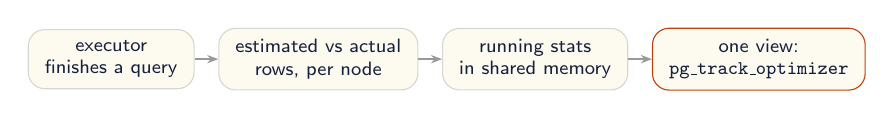
\begin{tikzpicture}[
  ptostep/.style={draw=mailrule, fill=paper, rounded corners=6pt, line width=0.4pt,
    inner xsep=6pt, inner ysep=4pt, font=\scriptsize\sffamily, text=ptoink,
    align=center},
  flow/.style={-{Stealth[length=4pt]}, black!40, line width=0.6pt}]
  \node[ptostep] (a) {executor\\finishes a query};
  \node[ptostep, right=0.3cm of a] (b) {estimated vs actual\\rows, per node};
  \node[ptostep, right=0.3cm of b] (c) {running stats\\in shared memory};
  \node[ptostep, right=0.3cm of c, draw=ptoaccent] (d) {one view:\\\ttfamily pg\_track\_optimizer};
  \draw[flow] (a) -- (b); \draw[flow] (b) -- (c); \draw[flow] (c) -- (d);
\end{tikzpicture}}

\vfill
\begin{tcbraster}[raster columns=2, raster equal height, raster column skip=0.5cm,
  raster row skip=0.35cm, enhanced, arc=3pt, colback=paper, boxrule=0.6pt,
  left=10pt, right=10pt, top=6pt, bottom=6pt]
\factcard{11}{metrics per query [ID]}
\factcard{0 restarts}{to start tracking: shared memory via the DSM registry, no preload needed}
\factcard{QueryID}{Modified Query ID to reduce the number of different entries}
\factcard{Persistent}{flushed to disk on backend exit, loaded back after a restart}
\end{tcbraster}
\vfill
\end{frame}

% %%%%%%%%%%%%%%%%%%%%%%%%%%%%%%%%%%%%%%%%%%%%%%%%%%%%%%%%%%%%%%%%%%%%%%%%
% Section divider: "Domain specifics" -- same pgEdge style as Chapters 1-2.
% Opens Nuances 1-3 and the design decisions they force.
% %%%%%%%%%%%%%%%%%%%%%%%%%%%%%%%%%%%%%%%%%%%%%%%%%%%%%%%%%%%%%%%%%%%%%%%%

\pgechapter{Chapter 3}{Domain specifics}

% %%%%%%%%%%%%%%%%%%%%%%%%%%%%%%%%%%%%%%%%%%%%%%%%%%%%%%%%%%%%%%%%%%%%%%%%
% Why the metrics are dimensionless: two plans that share nothing but
% the symptom. Numbers are copied from plans/dimensionless.raw.txt
% (PostgreSQL 18.6 release build; script plans/dimensionless.sql).
% %%%%%%%%%%%%%%%%%%%%%%%%%%%%%%%%%%%%%%%%%%%%%%%%%%%%%%%%%%%%%%%%%%%%%%%%

\begin{frame}\frametitle{Nuance 1: Queries are different}
\vspace{-0.6em}
\begin{columns}[T,onlytextwidth]

\begin{column}{0.60\textwidth}
\centering{\footnotesize\bfseries\color{ptoink}Two joins over a filtered scan}\par\smallskip\smallskip
\begin{forest} plangraph, for tree={font=\sffamily\tiny, inner xsep=2pt, l sep=16pt, s sep=4pt}
[Hash Join, rows={20}{20000}
  [Seq Scan, rows={100000}{100000}]
  [Hash, rows={1}{1000}
    [Nested Loop, detail={Removed: 4\,999\,000}, rows={1}{1000}, bad
      [Seq Scan, rows={1}{1000}]
      [Seq Scan, rows={5000}{5000}, loops={1000}]
    ]
  ]
]
\end{forest}

\smallskip{\scriptsize\color{black!55}6 nodes \textperiodcentered{} 2 joins \textperiodcentered{} 226\,ms}
\end{column}

\begin{column}{0.38\textwidth}
\centering{\footnotesize\bfseries\color{ptoink}GROUP BY over a scan}\par\smallskip\smallskip
\begin{forest} plangraph, for tree={font=\sffamily\tiny, inner xsep=2pt, l sep=16pt}
[HashAggregate, rows={2000}{100}, bad
  [Seq Scan, rows={20000}{20000}]
]
\end{forest}

\smallskip{\scriptsize\color{black!55}2 nodes \textperiodcentered{} 0 joins \textperiodcentered{} 1.4\,ms}
\end{column}

\end{columns}
\vfill
\end{frame}

% %%%%%%%%%%%%%%%%%%%%%%%%%%%%%%%%%%%%%%%%%%%%%%%%%%%%%%%%%%%%%%%%%%%%%%%%
% A node does not always run: one prepared statement, one generic plan,
% two executions. Numbers are copied from plans/never-executed.raw.txt
% (~/pg instance, REL_18_STABLE; script plans/never-executed.sql).
% %%%%%%%%%%%%%%%%%%%%%%%%%%%%%%%%%%%%%%%%%%%%%%%%%%%%%%%%%%%%%%%%%%%%%%%%

% one-line plan node for this slide: \nd{operator}{relation or condition}{actual rows}
\newcommand{\nd}[3]{#1\ifx\relax#2\relax\else\ \textcolor{planfade}{#2}\fi\enspace\textbf{#3}}

\begin{frame}[fragile]\frametitle{Nuance 2: Parameter might be in undefined state}
\vspace{-0.3em}
\begin{sql}[fontsize=\tiny]
PREPARE q(int, bool) AS
  SELECT o.id, p.id FROM orders o
    JOIN customers c ON c.id = o.cust JOIN payments p ON p.cust = c.id
  WHERE $1;
\end{sql}

\vfill

\begin{columns}[T,onlytextwidth]
\begin{column}{0.5\textwidth}
\centering{\scriptsize\bfseries\color{ptoink}\texttt{EXECUTE q(true)}}\par\smallskip\smallskip
\begin{forest} plangraph, for tree={font=\sffamily\tiny, inner xsep=1.5pt, inner ysep=1.5pt, l=0pt, l sep=12pt, s sep=2pt}
[{\nd{Result}{\$1}{20000}}, bad
  [{\nd{Hash Join}{}{20000}}
    [{\nd{Seq Scan}{payments}{100000}}]
    [{\nd{Hash}{}{1000}}
      [{\nd{Hash Join}{}{1000}}
        [{\nd{Seq Scan}{orders}{1000}}]
        [{\nd{Hash}{}{5000}}
          [{\nd{Seq Scan}{customers}{5000}}]
        ]
      ]
    ]
  ]
]
\end{forest}
\end{column}

\begin{column}{0.5\textwidth}
\centering{\scriptsize\bfseries\color{ptoink}\texttt{EXECUTE q(false)}}\par\smallskip\smallskip
\begin{forest} plangraph, for tree={font=\sffamily\tiny, inner xsep=1.5pt, inner ysep=1.5pt, l=0pt, l sep=12pt, s sep=2pt}
[{\nd{Result}{\$1}{0}}, bad
  [{\nd{Hash Join}{}{--}}, faded
    [{\nd{Seq Scan}{payments}{--}}, faded]
    [{\nd{Hash}{}{--}}, faded
      [{\nd{Hash Join}{}{--}}, faded
        [{\nd{Seq Scan}{orders}{--}}, faded]
        [{\nd{Hash}{}{--}}, faded
          [{\nd{Seq Scan}{customers}{--}}, faded]
        ]
      ]
    ]
  ]
]
\end{forest}
\end{column}
\end{columns}
\vfill
\end{frame}

% %%%%%%%%%%%%%%%%%%%%%%%%%%%%%%%%%%%%%%%%%%%%%%%%%%%%%%%%%%%%%%%%%%%%%%%%
% Estimation is stochastic: the data never change, only ANALYZE reruns.
% Counts come from plans/stochastic.csv (script plans/stochastic.sql,
% ~/pg instance, REL_18_STABLE, default_statistics_target = 100).
% %%%%%%%%%%%%%%%%%%%%%%%%%%%%%%%%%%%%%%%%%%%%%%%%%%%%%%%%%%%%%%%%%%%%%%%%

\begin{frame}[fragile]\frametitle{Nuance 3: statistics' stochastic nature}
\vspace{-0.3em}
\begin{sql}[fontsize=\small]
\sqlcmt{-- 40 times, the data never change}
\kw{ANALYZE} t;
\sqlcmt{-- actual: 10000 rows every time}
\kw{EXPLAIN} \kw{SELECT} * \kw{FROM} t \kw{WHERE} x = \sqlnum{77};
\end{sql}
\vspace{0.6em}
\begin{columns}[T,onlytextwidth]

\begin{column}{0.48\textwidth}
\begin{tcolorbox}[enhanced, arc=3pt, colback=paper, colframe=ptoink,
  boxrule=0.6pt, left=8pt, right=8pt, top=6pt, bottom=6pt,
  before skip=0pt, after skip=0pt, equal height group=stoch]
\small\color{ptoink}
\texttt{77} made it into the MCV list

\medskip
{\Large $\approx$\,10\,000} rows\\[2pt]
\textbf{Bitmap Heap Scan}

\medskip
{\scriptsize\color{black!55}21 runs of 40}
\end{tcolorbox}
\end{column}

\begin{column}{0.48\textwidth}
\begin{tcolorbox}[enhanced, arc=3pt, colback=paper, colframe=ptoink,
  boxrule=0.6pt, left=8pt, right=8pt, top=6pt, bottom=6pt,
  before skip=0pt, after skip=0pt, equal height group=stoch]
\small\color{ptoink}
\texttt{77} missed the MCV list

\medskip
{\Large $\approx$\,60} rows, \textcolor{crash}{\textbf{off by $\times$170}}\\[2pt]
\textbf{Index Scan}

\medskip
{\scriptsize\color{black!55}19 runs of 40}
\end{tcolorbox}
\end{column}

\end{columns}

\vfill
\end{frame}

% %%%%%%%%%%%%%%%%%%%%%%%%%%%%%%%%%%%%%%%%%%%%%%%%%%%%%%%%%%%%%%%%%%%%%%%%
% The answer to the three nuances: dimensionless metrics + the rstats type.
% Chips on top name the nuances from the previous three slides; arrows
% show which part of the design handles which nuance.
% %%%%%%%%%%%%%%%%%%%%%%%%%%%%%%%%%%%%%%%%%%%%%%%%%%%%%%%%%%%%%%%%%%%%%%%%

% card body: fixed-size top-aligned box, so both cards match
% units that cancel in a ratio, shown struck out in grey
\newcommand{\unitsgone}[2]{{\color{black!50}$\dfrac{\cancel{\text{#1}}}{\cancel{\text{#2}}}$}}
\newcommand{\cardbody}[1]{\parbox[t][4.6cm][t]{4.8cm}{\raggedright\hyphenpenalty=10000 #1}}
\tikzset{
  chip/.style={draw=mailrule, fill=paper, rounded corners=6pt, line width=0.4pt,
               inner xsep=6pt, inner ysep=3pt, text height=1.6ex, text depth=0.4ex,
               font=\scriptsize\sffamily, text=black!65},
  card/.style={draw=#1, fill=paper, rounded corners=3pt, line width=0.6pt,
               inner sep=6pt, anchor=north,
               font=\scriptsize\sffamily, text=ptoink},
  link/.style={-{Stealth[length=4pt]}, black!40, line width=0.6pt}}

\begin{frame}\frametitle{Two design decisions in pg\_track\_optimizer}
\vfill
\centering
\begin{tikzpicture}
  % the two parts of the answer
  \node[card=ptoink] (dim) at (-2.75, -0.75) {\cardbody{%
    {\center\small\bfseries Dimensionless metrics:}\par\medskip
    per plan node, units cancel out:\par\smallskip
     {\centering
      \begin{itemize}
        \item $e = \left|\,\ln\dfrac{\textit{actual rows}}{\textit{estimated rows}}\,\right|$
        \item $r = \dfrac{\textit{node time}}{\textit{total time}}$
        \item $f = \dfrac{\textit{filtered rows}}{\textit{actual rows}}$
        \item $b = \dfrac{\textit{local blocks}}{\textit{total blocks}}$
      \end{itemize}
      }\par\bigskip
    }};

  \node[card=ptoink] (rst) at (2.75, -0.75) {\cardbody{%
    {\center\small\bfseries Custom \texttt{RStats} type:}\par\medskip
    a distribution, not a number:\par\smallskip
    \centerline{\ttfamily (count, mean, min, max, stddev)}\par\smallskip
    \begin{itemize}
      \item Updated in place on every execution (Welford): the plan is unstable, not just wrong.\par
      \item The same code path for each parameter.
      \item Aggregate on statistic column.
    \end{itemize}
    }};
\end{tikzpicture}

  \vfill
\end{frame}

% %%%%%%%%%%%%%%%%%%%%%%%%%%%%%%%%%%%%%%%%%%%%%%%%%%%%%%%%%%%%%%%%%%%%%%%%
% Section divider: "How it works" -- same pgEdge style as Chapters 1-3.
% Opens the estimation-error method and the JOB walkthrough.
% %%%%%%%%%%%%%%%%%%%%%%%%%%%%%%%%%%%%%%%%%%%%%%%%%%%%%%%%%%%%%%%%%%%%%%%%

\pgechapter{Chapter 4}{How it works}

\begin{frame}\frametitle{How does it work in practice?}
\vspace{-0.4em}
{\large\sffamily\color{ptoink}Test bed: \textbf{the Join Order Benchmark}}\par
{\scriptsize\sffamily\color{black!45}Leis et al., \emph{How Good Are Query Optimizers, Really?}, PVLDB 2015}
\vfill
\begin{tcbraster}[raster columns=2, raster equal height, raster column skip=0.5cm,
  raster row skip=0.4cm, enhanced, arc=3pt, colback=paper, boxrule=0.6pt,
  left=10pt, right=10pt, top=8pt, bottom=8pt]
\factcard{113}{queries over real IMDb data}
\factcard{17}{tables joined in the deepest query}
\factcard{Scans}{many of them, including parameterised ones}
\factcard[ptoaccent]{Room}{plenty of it, for the planner to go wrong}
\end{tcbraster}
\vfill
\end{frame}

% %%%%%%%%%%%%%%%%%%%%%%%%%%%%%%%%%%%%%%%%%%%%%%%%%%%%%%%%%%%%%%%%%%%%%%%%
% The method in one picture (slide 11 of the PG Bootcamp deck, redrawn).
% Schematic plan, numbers from the original. e and the aggregates follow
% plan_error.c: e = |ln(act/est)|, avg = sum(e)/n, rms = sqrt(sum(e^2)/n).
% %%%%%%%%%%%%%%%%%%%%%%%%%%%%%%%%%%%%%%%%%%%%%%%%%%%%%%%%%%%%%%%%%%%%%%%%

\forestset{err/.style={content+={\\{\tiny\color{planfade}$e$ = #1}}}}

\begin{frame}\frametitle{Cardinality estimation error}
\vfill
\begin{columns}[T,onlytextwidth]

\begin{column}{0.54\textwidth}
\centering
\begin{forest} plangraph, for tree={font=\sffamily\scriptsize, l sep=22pt, s sep=10pt}
[Hash Join, rows={1000}{1200}
  [Nested Loop, rows={500}{480}
    [Index Scan, rows={50}{48}]
    [Seq Scan, rows={10}{12800}, bad]
  ]
  [Seq Scan, rows={2000}{2100}]
]
\end{forest}
\end{column}

\begin{column}{0.44\textwidth}
\small\color{ptoink}
\textbf{per-node error:}\par\smallskip
\centerline{$e = \left|\,\ln\dfrac{\textit{actual}}{\textit{estimated}}\,\right|$}\par

\bigskip\bigskip
\begin{tcolorbox}[enhanced, arc=3pt, colback=infobg, colframe=infoframe,
  boxrule=0.4pt, left=6pt, right=6pt, top=5pt, bottom=5pt,
  before skip=2pt, after skip=0pt]
{\scriptsize\color{ptoink} How to average across plan nodes?}
\end{tcolorbox}

%\vspace*{\fill}

\end{column}
\end{columns}

\vfill
\end{frame}

% %%%%%%%%%%%%%%%%%%%%%%%%%%%%%%%%%%%%%%%%%%%%%%%%%%%%%%%%%%%%%%%%%%%%%%%%
% How the criteria work on JOB (slides 13-14 of the PG Bootcamp deck).
% Images taken from 2026-PGBootcamp/pg_track_optimizer_presentation.pptx:
% image23.png -> pics/job-top10-avg-twa.png, image26.png -> pics/job-28a-depesz.png
% %%%%%%%%%%%%%%%%%%%%%%%%%%%%%%%%%%%%%%%%%%%%%%%%%%%%%%%%%%%%%%%%%%%%%%%%

\begin{frame}[fragile]\frametitle{How the estimation error criteria work}
\vspace{-0.4em}
{\small\color{ptoink}TOP-10 by average error V/S TOP-10 by time-weighted error}

\medskip
% was: pics/job-top10-avg-twa.png (screenshot); now live text
\begin{sql}[fontsize=\scriptsize]
\kw{SELECT} avg.* \kw{FROM}
  (\kw{SELECT} queryid, query, avg_avg, twa_avg \kw{FROM} pg_track_optimizer
   \kw{ORDER BY} avg_avg \kw{DESC} \kw{LIMIT} \sqlnum{10}) \kw{AS} avg
\kw{JOIN}
  (\kw{SELECT} queryid \kw{FROM} pg_track_optimizer
   \kw{ORDER BY} twa_avg \kw{DESC} \kw{LIMIT} \sqlnum{10}) \kw{AS} twa
\kw{USING} (queryid);
\end{sql}

\begin{psql}[fontsize=\scriptsize]
       queryid        |     query      | avg_avg | twa_avg
----------------------+----------------+---------+---------
\hl{ -6836119621424365027 | /* 28a.sql */  |    3.91 |    2.16}
  3631768377448547020 | /* 29c.sql */  |    3.77 |    2.51
 -8544699698054799639 | /* 22d.sql */  |    3.48 |    2.09
  4682104415514032107 | /* 7c.sql */   |    3.48 |    2.18
(4 rows)
\end{psql}
\end{frame}

\begin{frame}[fragile]\frametitle{A look inside 28a.sql}
\vspace{-0.5em}
\centering
% rows 12-22 of the depesz view: the red cells and the yellow x94.7 node
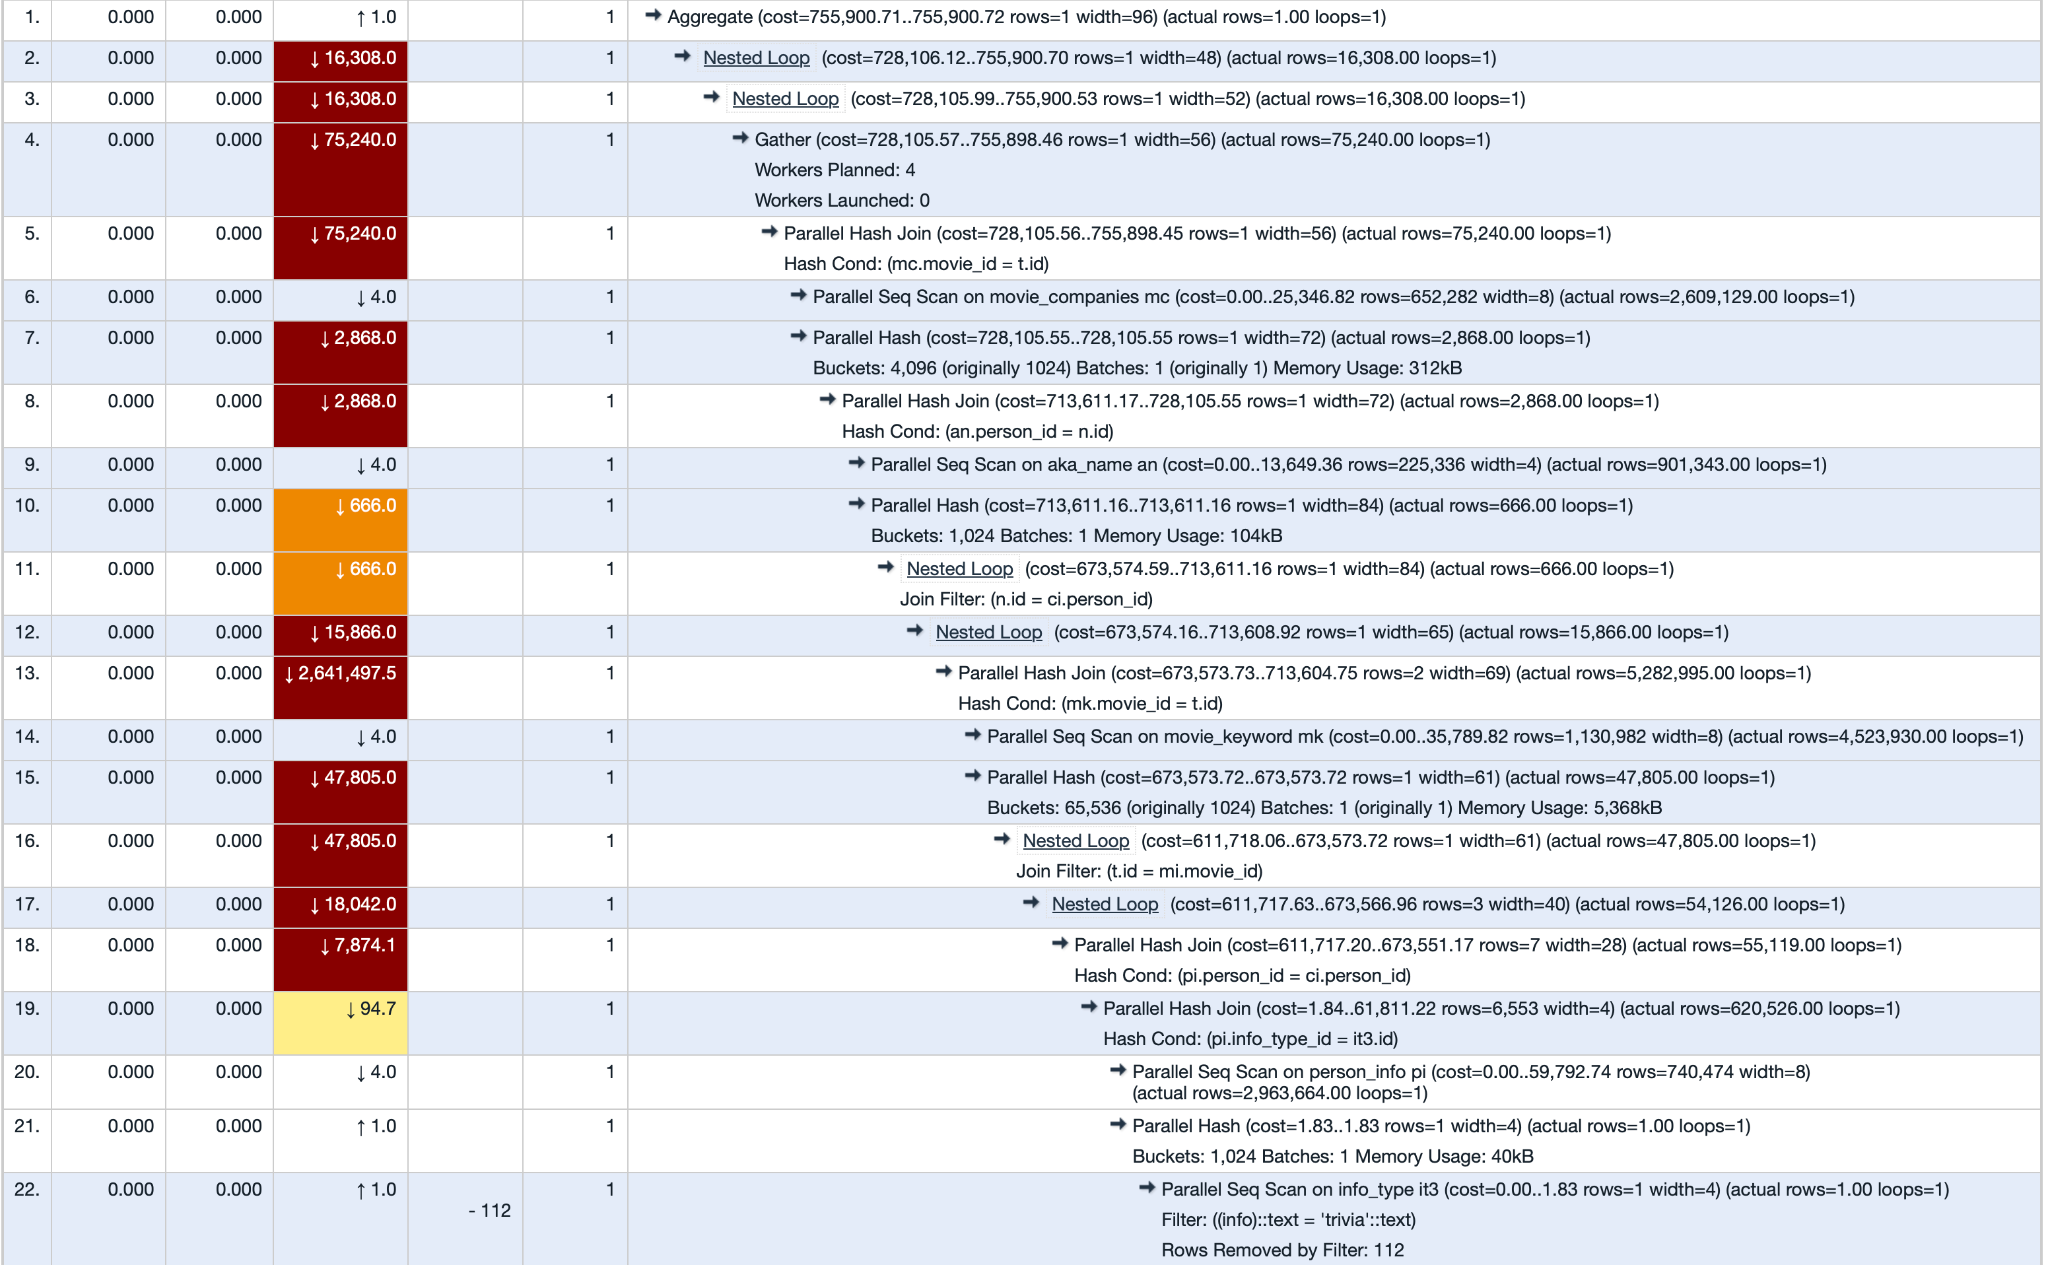
\includegraphics[width=\textwidth, trim=0 0 0 612, clip]{pics/job-28a-depesz.png}

\raggedright
\begin{plan}[fontsize=\tiny]
->  Parallel Hash Join \hl{(rows=6553) (actual rows=620526)}
      Hash Cond: (pi.info_type_id = it3.id)
      ->  Parallel Seq Scan on person_info pi \hl{(rows=740474) (actual rows=2963664)}
      ->  Parallel Hash (rows=1) (actual rows=1.00)
            ->  Parallel Seq Scan on info_type it3 (rows=1) (actual rows=1)
                  Filter: ((info)::text = 'trivia'::text)
                  Rows Removed by Filter: 112
\end{plan}
\takeaway{The x4 scan error grows throughout the join tree.}
\end{frame}

% %%%%%%%%%%%%%%%%%%%%%%%%%%%%%%%%%%%%%%%%%%%%%%%%%%%%%%%%%%%%%%%%%%%%%%%%
% Criterion 2: filter factors (slides 16-17 of the PG Bootcamp deck, merged).
% Formulas follow plan_error.c: scans take nfiltered1, joins take
% nfiltered1 + nfiltered2; both are per loop, divided by actual rows and
% weighted by node time / total time; the query keeps the maximum.
% The plan is schematic. The Bootcamp original had "Filter: c.segment" on
% the Hash Join, which the planner would push down to the customers scan;
% here it is a Join Filter that cannot be pushed, and the counts add up:
% 289 + 47542 = 47831 rows from orders.
% %%%%%%%%%%%%%%%%%%%%%%%%%%%%%%%%%%%%%%%%%%%%%%%%%%%%%%%%%%%%%%%%%%%%%%%%

\colorlet{scanhl}{ptoteal!22}
\colorlet{joinhl}{ptoaccent!22}
\newcommand\hls[1]{{\setlength\fboxsep{0pt}\colorbox{scanhl}{\strut#1}}}
\newcommand\hlj[1]{{\setlength\fboxsep{0pt}\colorbox{joinhl}{\strut#1}}}

\begin{frame}[fragile]\frametitle{Filter factors: scans and joins}
\begin{tcolorbox}[enhanced, arc=3pt, colback=paper, colframe=ptoteal,
  boxrule=0.6pt, left=6pt, right=6pt, top=3pt, bottom=3pt,
  before skip=0pt, after skip=4pt]
\parbox[c]{2.0cm}{\raggedright {\scriptsize\bfseries\color{ptoteal}Scans}\par}%
\hfill\mbox{\small\color{ptoink}$\displaystyle f_{\mathit{scan}} = \max_{\mathit{scans}}
  \biggl(\frac{\colorbox{scanhl}{\strut\textit{removed by filter}}}{\textit{actual rows}}
  \times\frac{\textit{node time}}{\textit{total time}}\biggr)$}\hfill\null
\end{tcolorbox}
\begin{tcolorbox}[enhanced, arc=3pt, colback=paper, colframe=ptoaccent,
  boxrule=0.6pt, left=6pt, right=6pt, top=3pt, bottom=3pt,
  before skip=0pt, after skip=4pt]
\parbox[c]{2.0cm}{\raggedright {\scriptsize\bfseries\color{ptoteal}Joins}\par}%
\hfill\mbox{\small\color{ptoink}$\displaystyle f_{\mathit{join}} = \max_{\mathit{joins}}
  \biggl(\frac{\colorbox{joinhl}{\strut\textit{removed by join filter}}}{\textit{actual rows}}
  \times\frac{\textit{node time}}{\textit{total time}}\biggr)$}\hfill\null
\end{tcolorbox}

\begin{plan}[fontsize=\scriptsize]
Hash Join  (actual time=234.671 rows=\hlj{289} loops=1)
  Hash Cond: (o.customer_id = c.id)
  Join Filter: (o.amount > c.credit_limit)
  \hlj{Rows Removed by Join Filter: 47542}
  ->  Seq Scan on orders o  (actual time=98.341 rows=\hls{47831} loops=1)
        Filter: (status = 'completed')
        \hls{Rows Removed by Filter: 952169}
  ->  Hash  (actual time=42.110 rows=100000 loops=1)
        ->  Seq Scan on customers c  (actual time=21.543 rows=100000)
\end{plan}
\end{frame}

% %%%%%%%%%%%%%%%%%%%%%%%%%%%%%%%%%%%%%%%%%%%%%%%%%%%%%%%%%%%%%%%%%%%%%%%%
% How the scan filter factor works on JOB (slide 18 of the PG Bootcamp
% deck). Two overlays, used as a two-step animation:
%   <1> TOP-5 by lf_avg + the depesz heatmap of 15b.sql;
%   <2> the same, plus the movie_info scan (heatmap row 18) boxed in red
%       and magnified as EXPLAIN text.
% Numbers from 2026-PGBootcamp/pg_track_optimizer_presentation.pptx:
% image29.png (the table; view renamed track_data -> pg_track_optimizer),
% image30.jpg -> pics/job-15b-heatmap.jpg (1072 x 1048 px).
% EXPLAIN shows Rows Removed by Filter per loop, like actual rows:
% 2 966 790 / 354.2 ~ 8 376 rows discarded per row returned.
% %%%%%%%%%%%%%%%%%%%%%%%%%%%%%%%%%%%%%%%%%%%%%%%%%%%%%%%%%%%%%%%%%%%%%%%%

% the magnified fragment, typeset once outside the frame (verbatim cannot
% live inside a TikZ node)
\newsavebox\zoomplan
\begin{lrbox}{\zoomplan}\begin{minipage}{0.93\textwidth}
\begin{plan}[fontsize=\tiny]
->  Parallel Hash Join (actual rows=354.20 loops=5)
      Hash Cond: (mi.info_type_id = it1.id)
      ->  Parallel Seq Scan on movie_info mi \hl{(actual rows=354.20 loops=5)}
            Filter: ((note ~~ '%internet%'::text) AND (info ~~ 'USA:% 200%'::text))
            \hl{Rows Removed by Filter: 2966790}
      ->  Parallel Hash (actual rows=0.20 loops=5)
\end{plan}
\end{minipage}\end{lrbox}

\begin{frame}[fragile,t]\frametitle{How the filter criteria work}
\begin{columns}[T,onlytextwidth]
\begin{column}{0.62\textwidth}
\begin{sql}[fontsize=\tiny]
\kw{SELECT} queryid, query, avg_avg, lf_avg
\kw{FROM} pg_track_optimizer
\kw{ORDER BY} lf_avg \kw{DESC} \kw{LIMIT} \sqlnum{5};
\end{sql}

\begin{psql}[fontsize=\tiny]
       queryid        |     query     | avg_avg | lf_avg
----------------------+---------------+---------+---------
\hl{  7987931480126446697 | /* 15b.sql */ |    1.60 | 1459.35}
 -4244378222084090458 | /* 23a.sql */ |    1.75 | 1424.58
 -6679854959453081533 | /* 15a.sql */ |    1.95 | 1406.36
 -1139306376856509831 | /* 23b.sql */ |    1.48 | 1403.23
 -4904731422305343909 | /* 15c.sql */ |    2.69 | 1342.81
(5 rows)
\end{psql}
\end{column}

\begin{column}{0.36\textwidth}
\centering
\begin{tikzpicture}[remember picture]
  \node[inner sep=0pt, anchor=south west, draw=mailrule, line width=0.4pt] (heat) at (0,0)
    {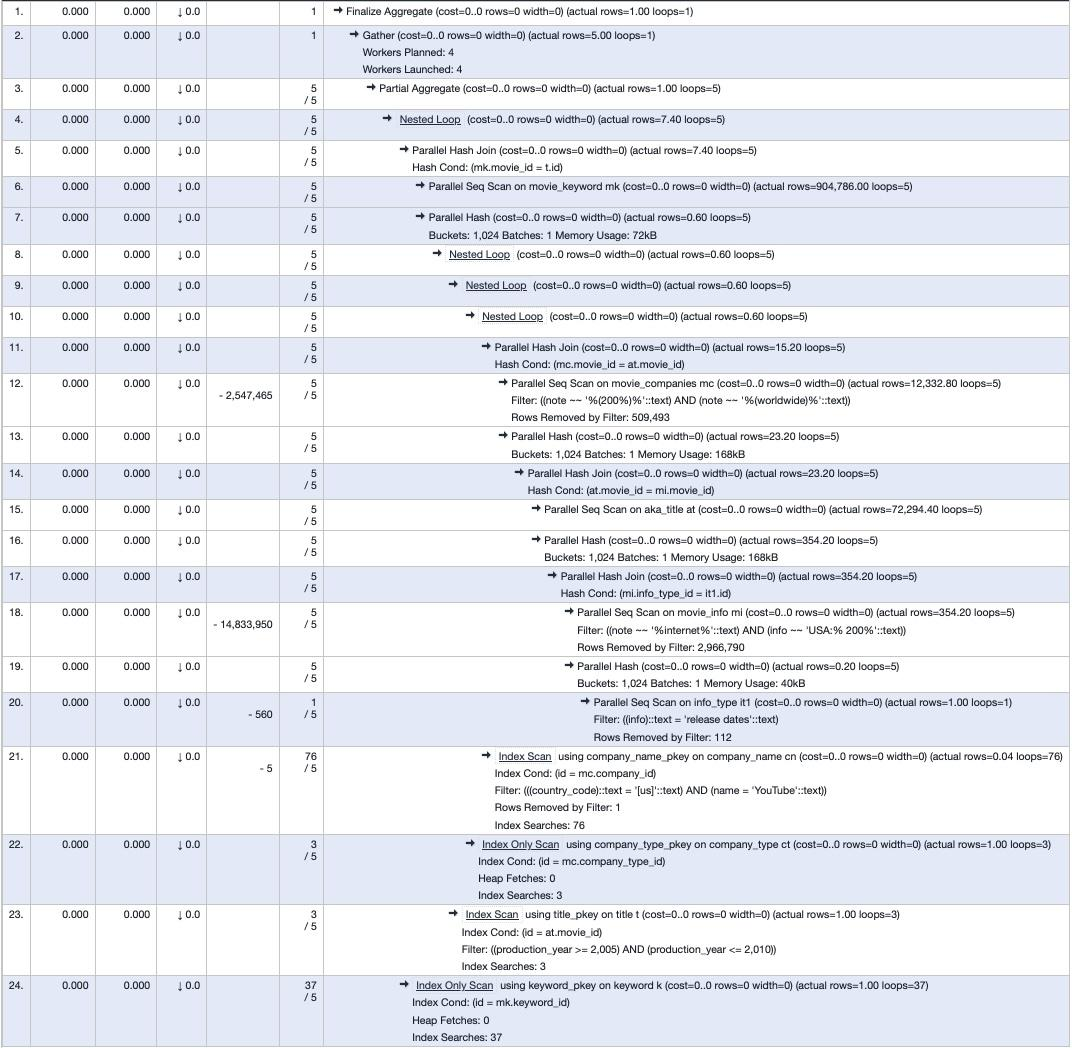
\includegraphics[width=\linewidth]{pics/job-15b-heatmap.jpg}};
  % row 18 of the heatmap: y = 603..656 px of 1048
  \begin{scope}[x={(heat.south east)}, y={(heat.north west)}]
    \coordinate (hotSW) at (0, 0.374);
    \only<2>{\draw[crash, line width=1pt] (0, 0.374) rectangle (1, 0.425);}
  \end{scope}
\end{tikzpicture}
\end{column}
\end{columns}

\only<2>{%
\begin{tikzpicture}[remember picture, overlay]
  \node[anchor=south west, inner sep=0pt, draw=crash, line width=1pt, fill=white]
    (zoom) at ([xshift=0.3cm, yshift=1.3cm]current page.south west) {\usebox\zoomplan};
  \draw[crash, line width=0.8pt] (hotSW) -- (zoom.north east);
\end{tikzpicture}}
\end{frame}

% %%%%%%%%%%%%%%%%%%%%%%%%%%%%%%%%%%%%%%%%%%%%%%%%%%%%%%%%%%%%%%%%%%%%%%%%
% Effect of the indexes the filter factors pointed at (slide 21 of the
% PG Bootcamp deck, redrawn). Data: plans/job-speedup.dat, built from
% 2026-PGBootcamp/job-indexes/job-{plain,scan-index,join-index}.txt.
% The original plotted speedup per query, linear axis capped at 30.
% Here each series is sorted (rank plot) on a log axis, so gains and
% regressions get the same room. Totals over 113 queries:
% plain 66.7 s, scan indexes 66.6 s, join indexes 64.2 s.
% %%%%%%%%%%%%%%%%%%%%%%%%%%%%%%%%%%%%%%%%%%%%%%%%%%%%%%%%%%%%%%%%%%%%%%%%

\begin{frame}\frametitle{Effect of the indexes found}
\centering
\begin{tikzpicture}
\begin{axis}[
  width=0.98\textwidth, height=0.62\textheight,
  ymode=log, log basis y=10, ymin=0.05, ymax=400,
  xmin=0, xmax=114,
  ytick={0.1,1,10,100}, yticklabels={×0.1,×1,×10,×100},
  xtick={1,20,40,60,80,100,113}, xticklabels={1,20,40,60,80,100,113},
  xlabel={queries, sorted by speedup}, ylabel={speedup},
  label style={font=\scriptsize\sffamily, text=black!55},
  tick label style={font=\scriptsize\sffamily, text=black!55},
  axis line style={black!35}, tick style={black!35},
  axis x line*=bottom, axis y line*=left,
  ymajorgrids, grid style={black!8},
  clip=false]
  \addplot[black!45, dashed, thin, domain=0:114, samples=2] {1};
  \addplot[ptoaccent, line width=1.1pt] table[x=rank, y=join] {plans/job-speedup.dat};
  \addplot[ptoteal, line width=1.1pt] table[x=rank, y=scan] {plans/job-speedup.dat};
  % direct labels instead of a legend
  \node[font=\scriptsize\sffamily\bfseries, text=ptoaccent, anchor=west] at (axis cs:12,40) {join indexes};
  \node[font=\scriptsize\sffamily\bfseries, text=ptoteal, anchor=north west] at (axis cs:10,0.75) {scan indexes};
  % the extremes
  \node[font=\tiny\sffamily, text=ptoink, anchor=west] at (axis cs:2,196) {12b: $\times$196};
  \node[font=\tiny\sffamily, text=ptoink, anchor=east] at (axis cs:111,0.07) {26c, 33a: $\times$0.07};
  \node[font=\tiny\sffamily, text=black!55, anchor=south east] at (axis cs:113,1) {no change};
\end{axis}
\end{tikzpicture}

\par\smallskip
{\small\color{ptoink}JOB, 113 queries: plain time / time with the new indexes, best to worst\par}
\end{frame}

% %%%%%%%%%%%%%%%%%%%%%%%%%%%%%%%%%%%%%%%%%%%%%%%%%%%%%%%%%%%%%%%%%%%%%%%%
% Join-filtered rows that vanilla EXPLAIN does not show.
% big: 10^7 rows, 64-byte tuples; only 1000 of them (one contiguous block,
% 12 heap pages) have x in 1..10. small: 100 rows, x = 1..100, only 10 have
% a partner. Result: 1000 rows; 9 999 000 rows of big and 90 rows of small
% are thrown away by the join. No indexes.
% Right column: the same query as Hash Join (planner's choice) and as a
% forced Nested Loop (enable_hashjoin = enable_mergejoin = off).
%   Hash Join -- says nothing about the rows it threw away;
%   Nested Loop -- Rows Removed by Join Filter = 10^7 x 100 - 1000 compared
%   PAIRS, not rows without a partner.
% Plans trimmed for the slide: Buffers, Planning, Buckets/Memory and
% Materialize Storage lines removed; the rest verbatim from
% plans/join-big-small-dense-noindex.raw.txt and
% plans/join-big-small-dense-nl-noindex.raw.txt (script:
% plans/join-big-small-dense.sql; PG 18.6, no parallel workers).
% %%%%%%%%%%%%%%%%%%%%%%%%%%%%%%%%%%%%%%%%%%%%%%%%%%%%%%%%%%%%%%%%%%%%%%%%

\begin{frame}[fragile,t]\frametitle{Join filtering EXPLAIN can't see}
\vfill
\begin{columns}[T,onlytextwidth]

\begin{column}{0.33\textwidth}
\centering
\begin{forest} plangraph
[Join, detail={big.x = small.x}, act={1000 rows}, l sep=30pt, s sep=26pt
  [big, act={$10^7$ rows},
   edge label={node[midway, left, inner sep=3pt, align=right,
     font=\sffamily\tiny\bfseries, text=planbad]{}}]
  [small, act={100 rows},
   edge label={node[midway, right, inner sep=3pt, align=left,
     font=\sffamily\tiny\bfseries, text=planbad]{}}]]
\end{forest}

\vspace{5mm}
\begin{sql}[fontsize=\tiny]
\kw{SELECT} * \kw{FROM} big
  \kw{JOIN} small \kw{USING} (x);
\end{sql}

\end{column}

\begin{column}{0.65\textwidth}
{\sffamily\scriptsize\bfseries\color{ptoink}Hash Join\par}
\begin{plan}[fontsize=\tiny]
Hash Join (actual rows=1000.00 loops=1)
  Hash Cond: (big.x = small.x)
  ->  Seq Scan on big (actual rows=10000000.00 loops=1)
  ->  Hash (actual rows=100.00 loops=1)
        ->  Seq Scan on small (actual rows=100.00 loops=1)
Execution Time: 332.203 ms
\end{plan}

\bigskip\bigskip
{\sffamily\scriptsize\bfseries\color{ptoink}Nested Loop\par}
\begin{plan}[fontsize=\tiny]
Nested Loop (actual rows=1000.00 loops=1)
  Join Filter: (big.x = small.x)
  \hl{Rows Removed by Join Filter: 999999000}
  ->  Seq Scan on big (actual rows=10000000.00 loops=1)
  ->  Materialize (actual rows=100.00 loops=10000000)
        ->  Seq Scan on small (actual rows=100.00 loops=1)
Execution Time: 20799.413 ms
\end{plan}
\end{column}

\end{columns}
\vfill
\end{frame}

% %%%%%%%%%%%%%%%%%%%%%%%%%%%%%%%%%%%%%%%%%%%%%%%%%%%%%%%%%%%%%%%%%%%%%%%%
% Same slide, second step: the Nested Loop box is replaced by the plan
% with an index on big(x) (forced Nested Loop, CREATE INDEX big_x_idx),
% framed in red. rows=10.00 loops=100 is an average: 90 probes return
% nothing, 10 return 100 rows each -- EXPLAIN can't tell them apart.
% Trimmed like the previous slide (Buffers, Planning removed); source:
% plans/join-big-small-dense-nl-index.raw.txt.
% %%%%%%%%%%%%%%%%%%%%%%%%%%%%%%%%%%%%%%%%%%%%%%%%%%%%%%%%%%%%%%%%%%%%%%%%

\begin{frame}[fragile,t]\frametitle{Join filtering EXPLAIN can't see}
\vfill
\begin{columns}[T,onlytextwidth]

\begin{column}{0.33\textwidth}
\centering
\begin{forest} plangraph
[Join, detail={big.x = small.x}, act={1000 rows}, l sep=30pt, s sep=26pt
  [big, act={$10^7$ rows},
   edge label={node[midway, left, inner sep=3pt, align=right,
     font=\sffamily\tiny\bfseries, text=planbad]{}}]
  [small, act={100 rows},
   edge label={node[midway, right, inner sep=3pt, align=left,
     font=\sffamily\tiny\bfseries, text=planbad]{}}]]
\end{forest}

\vspace{5mm}
\begin{sql}[fontsize=\tiny]
\kw{SELECT} * \kw{FROM} big
  \kw{JOIN} small \kw{USING} (x);
\end{sql}
\begin{planhot}[fontsize=\tiny]
\kw{CREATE INDEX} idx \kw{ON} big (x);
\end{planhot}

\end{column}

\begin{column}{0.65\textwidth}
{\sffamily\scriptsize\bfseries\color{ptoink}Hash Join\par}
\begin{plan}[fontsize=\tiny]
Hash Join (actual rows=1000.00 loops=1)
  Hash Cond: (big.x = small.x)
  ->  Seq Scan on big (actual rows=10000000.00 loops=1)
  ->  Hash (actual rows=100.00 loops=1)
        ->  Seq Scan on small (actual rows=100.00 loops=1)
Execution Time: 332.203 ms
\end{plan}

\bigskip\bigskip
{\sffamily\scriptsize\bfseries\color{ptoink}Nested Loop\par}
\begin{planhot}[fontsize=\tiny]
Nested Loop (actual rows=1000.00 loops=1)
  ->  Seq Scan on small (actual rows=100.00 loops=1)
  ->  Index Scan using idx on big
        (actual rows=\hl{10.00 loops=100})
        Index Cond: (x = small.x)
        Index Searches: 100
Execution Time: 0.187 ms
\end{planhot}
\end{column}

\end{columns}
\vfill
\end{frame}

% %%%%%%%%%%%%%%%%%%%%%%%%%%%%%%%%%%%%%%%%%%%%%%%%%%%%%%%%%%%%%%%%%%%%%%%%
% Spilling of intermediate results -- the setup slide (slide 26 of the PG
% Bootcamp deck), placed right before the live demo. Lists which plan
% nodes can spill once they outgrow work_mem, and how pg_track_optimizer
% detects it (local_blks). Text adapted from the Bootcamp slide; its
% screenshot was the same ranking query shown live on the next slide, so
% it is not repeated here.
% %%%%%%%%%%%%%%%%%%%%%%%%%%%%%%%%%%%%%%%%%%%%%%%%%%%%%%%%%%%%%%%%%%%%%%%%

\begin{frame}\frametitle{Spilling of intermediate results}
  \vspace*{\fill}
  \begin{columns}[T,onlytextwidth]
    \begin{column}{0.5\textwidth}
      {\large\color{ptoink}Who spills:}\medskip
      {\small\color{ptoink}
        \begin{itemize}\itemsep4pt
          \item Hash Join
          \item Hash Aggregate
          \item Window Aggregate
          \item Sort
          \item Materialize
          \item CTE /Recursive CTE
        \end{itemize}
      }
  \end{column}
    
    \begin{column}{0.5\textwidth}
       {\large\color{ptoink}Who doesn't spill:}\medskip
      {\small\color{ptoink}
        \begin{itemize}\itemsep4pt
          \item INTERSECT/EXCEPT (Hashed)
          \item Memoize
          \item Hashed SubPlan
          \item BitmapScan
        \end{itemize}
      }
    \end{column}
  \end{columns}
  \vspace*{\fill}
\end{frame}

% %%%%%%%%%%%%%%%%%%%%%%%%%%%%%%%%%%%%%%%%%%%%%%%%%%%%%%%%%%%%%%%%%%%%%%%%
% Spilling of intermediate results (lever 4 of "Assessing the instance's
% potential"), adapted from slide 27 of the PG Bootcamp deck: the ranking
% query (screenshot on slide 26, carried over onto slide 27) plus the live
% work_mem demo (slide 27's own text box). Both rendered as live text with
% highlighting, by analogy with the estimation-error and filter-factor
% criteria above -- not as a screenshot.
% Query and numbers copied verbatim from the Bootcamp slides.
% %%%%%%%%%%%%%%%%%%%%%%%%%%%%%%%%%%%%%%%%%%%%%%%%%%%%%%%%%%%%%%%%%%%%%%%%

\begin{frame}[fragile]\frametitle{How the spilling criterion works}
\vspace{-0.4em}
{\small\color{ptoink}Rank queries by how much they spill, then see if memory actually matters}

\medskip
\begin{columns}[T,onlytextwidth]

\begin{column}{0.54\textwidth}
\begin{sql}[fontsize=\tiny]
\kw{SELECT} queryid, \kw{LEFT}(query,\sqlnum{13}) \kw{AS} query,
  \kw{ROUND}((temp_avg*\sqlnum{8192}/\sqlnum{1024}/\sqlnum{1024})
    ::numeric,\sqlnum{0}) \kw{AS} spill_mb
\kw{FROM} track_data
\kw{ORDER BY} \kw{CASE WHEN} blks_avg = \sqlnum{0} \kw{THEN} \sqlnum{0}
  \kw{ELSE} temp_avg/blks_avg \kw{END} \kw{DESC}
\kw{LIMIT} \sqlnum{5};
\end{sql}

\begin{psql}[fontsize=\tiny]
      queryid         |    query     | spill_mb
----------------------+--------------+----------
\hl{ -4733402157366146115 | /* 8c.sql */  |      598}
 -3437698612165670854 | /* 8d.sql */  |      381
  4682104415514032107 | /* 7c.sql */  |     2678
  1798119524484989875 | /* 10c.sql */ |      179
 -3013169471333993680 | /* 16c.sql */ |       91
(5 rows)
\end{psql}
\end{column}

\begin{column}{0.42\textwidth}
\centering{\scriptsize\bfseries\color{ptoink}Same query, only work\_mem changes}\par\smallskip
\begin{psql}[fontsize=\scriptsize]
\kw{SET} work_mem = '1MB';
Execution Time: \hl{1841} ms

\kw{SET} work_mem = '4MB';
Execution Time: \hl{1405} ms

\kw{SET} work_mem = '64MB';
Execution Time: \hl{950} ms
\end{psql}
\end{column}

\end{columns}
\end{frame}

% %%%%%%%%%%%%%%%%%%%%%%%%%%%%%%%%%%%%%%%%%%%%%%%%%%%%%%%%%%%%%%%%%%%%%%%%
% What raising work_mem changes in the plan (slide 28 of the PG Bootcamp
% deck), closing the setup -> demo -> consequences arc for the spilling
% criterion. Eight plan-shape swaps the planner makes once memory stops
% being the limiting factor, plus the closing remark about plans growing
% more aggressive and more error-sensitive. Node names spelled out in full
% (Nested Loop, Group Aggregate, ...) to match this deck's own convention,
% rather than the Bootcamp slide's abbreviations (NestLoop, GroupAgg).
% Bold items match the Bootcamp deck's own emphasis.
% %%%%%%%%%%%%%%%%%%%%%%%%%%%%%%%%%%%%%%%%%%%%%%%%%%%%%%%%%%%%%%%%%%%%%%%%

\begin{frame}\frametitle{What a bigger \texttt{work\_mem} changes}
\vspace*{\fill}

{\small\color{ptoink}
\begin{itemize}\itemsep6pt
  \item \textbf{Hash Join $\rightarrow$ Nested Loop + Memoize}
  \item Incremental Sort + Merge Append $\rightarrow$ Sort + Append
  \item Merge Append + Sort $\rightarrow$ Sort + Append
  \item \textbf{Group Aggregate + Sort $\rightarrow$ Hash Aggregate}
  \item Index Scan $\rightarrow$ Sort + Seq Scan
  \item Index Scan $\rightarrow$ Incremental Sort + Index Scan
  \item \textbf{Hash Join $\rightarrow$ Merge Join}
  \item $\rightarrow$ Materialize
\end{itemize}}

\vspace*{\fill}
\end{frame}

% %%%%%%%%%%%%%%%%%%%%%%%%%%%%%%%%%%%%%%%%%%%%%%%%%%%%%%%%%%%%%%%%%%%%%%%%
% Section divider: "Outcomes" -- same pgEdge style as Chapters 1-4.
% The parenthetical is a smaller, lighter second line so the joke reads
% as an aside, not as part of the title.
% %%%%%%%%%%%%%%%%%%%%%%%%%%%%%%%%%%%%%%%%%%%%%%%%%%%%%%%%%%%%%%%%%%%%%%%%

\pgechapter{Chapter 5}{Outcomes\\[3mm]{\fontsize{16}{19}\selectfont\mdseries\spaceskip=0pt\color{pgePath}(the shortest one)}}

% %%%%%%%%%%%%%%%%%%%%%%%%%%%%%%%%%%%%%%%%%%%%%%%%%%%%%%%%%%%%%%%%%%%%%%%%
% What to monitor (slide 36 of the PG Bootcamp deck, translated). Same
% \lever layout as "Assessing the instance's potential": metric, then what
% a change in it may mean. Items 1-3 follow the original; the original had
% no explanation for item 4, its second line is new.
% %%%%%%%%%%%%%%%%%%%%%%%%%%%%%%%%%%%%%%%%%%%%%%%%%%%%%%%%%%%%%%%%%%%%%%%%

\begin{frame}\frametitle{The useful bits}
\vspace*{\fill}

\lever{1}{Track accumulated average error}
  {On tuned system growth or spike in average error means loosing efficiency}
\lever{2}{Watch SCAN and JOIN Filter factors}
  {The most critical metrics that expose missed indexes}
\lever{3}{Combine these metrics with \texttt{pg\_stat\_statements}}
  {It might highlight queries that deserve GENERIC/CUSTOM plan changeover}

\vspace*{\fill}
\end{frame}

% %%%%%%%%%%%%%%%%%%%%%%%%%%%%%%%%%%%%%%%%%%%%%%%%%%%%%%%%%%%%%%%%%%%%%%%%
% Closing slide. Short on purpose -- a contact card, not a "thank you"
% slide. QR code is rendered live by the qrcode package rather than pasted
% in as an image. Points at the pg_track_optimizer repo so people can scan
% and go straight to the source. E-mail is personal by convention.
% %%%%%%%%%%%%%%%%%%%%%%%%%%%%%%%%%%%%%%%%%%%%%%%%%%%%%%%%%%%%%%%%%%%%%%%%

% pgEdge-style closing: navy canvas, matching the cover (bookends), contacts
% as plain lines (not bullets), QR on a white card so phones still scan it.
{\setbeamertemplate{background}{%
  \begin{tikzpicture}[x=1pt,y=1pt]
    \useasboundingbox (0,0) rectangle (\paperwidth,\paperheight);
    \fill[pgeNavy] (0,0) rectangle (\paperwidth,\paperheight);
    \node[anchor=east,inner sep=0,opacity=0.3] at ([xshift=18mm]\paperwidth,0.5\paperheight)
      {
\includegraphics[height=\paperheight]{pgedge-assets/ascii-elephant-head-light}};
    \node[anchor=west,inner sep=0,text width=0.58\paperwidth,align=left]
      at (7mm,0.5\paperheight) {%
      {\sffamily\bfseries\fontsize{32}{32}\selectfont\color{white}%
       \spaceskip=0.32em\relax Questions?\par}%
      \vskip9mm
      {\sffamily\bfseries\fontsize{12}{14}\selectfont\color{white}Andrei Lepikhov\par}%
      \vskip1mm
      {\sffamily\fontsize{10}{12}\selectfont\color{pgeSkyMid}pgEdge\par}%
      \vskip5mm
      {\sffamily\fontsize{8.5}{12}\selectfont\color{pgeSkyMid}%
       lepihov@gmail.com\par github.com/danolivo\par pgedge.com\par}};
    \node[anchor=east,inner sep=3.2mm,fill=white,rounded corners=1.2mm,align=center]
      at ([xshift=-9mm]\paperwidth,0.5\paperheight) {%
      \qrcode[height=2.8cm]{https://github.com/danolivo/pg_track_optimizer}\\[2mm]
      {\sffamily\fontsize{6.5}{8}\selectfont\color{pgeNavy}pg\_track\_optimizer on GitHub}};
  \end{tikzpicture}}%
\begin{frame}[plain]\end{frame}}

\end{document}
